Монады в Yesod

Как вы уже увидели в этой книге появилось несколько монад: Handler, Widget и YesodDB (для пакета Persistant). Как и всякая монада, каждая из них предоставляет некоторую специфическцю функциональность: Handler предоставляет доступ к запросу и позволяет отправлять ответы, Widget содержит HTML, CSS и Javascript, а YesodDB позволяет делать запросы к базе данных. В терминах Model-View-Controller (MVC), мы могли бы рассматривать YesodDB как модель, Widget как представление, и Handler как контроллер.

До сих пор у нас представлены очень простые способы использования этих монад: основной обработчик работает в Handler, используя runDB для выполнения запроса YesodDB и defaultLayout для возврата Widget, который в свою очередь был создан вызовом toWidget.

Тем не менее, если у нас будет глубокое понимание этих типов, мы сможем достичь более интересных результатов.

Трансформеры Монад

Монады они как луковицы. Монады не как пироженные. Вроде бы Шрек.

Прежде чем попасть в сердце монад Yesod, мы должны немного понимать о трансформере монад. (Если вы уже всё знаете о трансформере монад, вы, скорее всего, можете пропустить этот раздел.) Различные монады предоставляют различную функциональность: Reader позволяет доступ только для чтения к некоторым данных по всему вычислению, Error позволяет оборвать, и так далее.

Однако, часто вы захотите иметь возможность объединить несколько из этих функций вместе. В конце концов, почему бы не иметь вычисления с доступом только для чтения для некоторых переменных, которые могли бы ошибиться в любое время? Одним из подходов к этому было бы написать новую монаду, например ReaderError, но это имеет очевидный недостаток экспоненциальной сложности: нужно написать новую монаду для каждой возможной комбинации.

Вместо этого у нас есть трансформеры монад. В дополнение к Reader, у нас есть ReaderT, который добавляет функциональность Reader к любой другой монаде. Таким образом, мы могли бы представить нашу ReaderError как (концептуально):

\begin{lstlisting}
type ReaderError = ReaderT Error
\end{lstlisting}

Чтобы получить доступ к нашим параметрам настройки, мы можем использовать функцию запроса (ask). А как насчет обрыввания вычисления? Мы хотели бы использовать throwError, но это не будет как следует работать. Вместо этого мы должны поднять (lift) наш вызов в монаду на уровень выше. Другими словами:

\begin{lstlisting}
throwError :: errValue -> Error
lift . throwError :: errValue -> ReaderT Error
\end{lstlisting}

Есть несколько вещей, которые вы должны здесь понять:

* Трансформер может быть использован для добавления функциональных возможностей в существующие монады.
* Трансформер должен всегда обертываться вокруг существующей монады.
* Функциональные возможности получившейся монады будут зависеть не только от трансформера монады, но и от монады обёрнутой внутри.

Отличный пример последнего утверждения это монада IO. Независимо от того, сколько слоев трансформеров у вас есть вокруг IO, там всё ещё есть ядро IO, то есть вы можете выполнять I/O в любом из этих стеков этих трансформеров монад. Вы будете часто видеть код, который выглядит как \lstinline'liftIO $ putStrLn "Hello There!"'.

Три Трансформера

Мы уже обсуждали два наших трансформатора ранее: Handler и Widget. Просто напомним, есть два специальных факта об этих трансформеров:

1) В целях упрощения сообщений об ошибках, они не являются фактическими трансформерами. Вместо этого, они являются новыми типами (newtypes) с реализацией своей внутренней монады. Помните, что это поэтому Yesod предоставляет специальную функцию подъёма (lift), которая работает для Handler и Widget.
2) На самом деле у них есть дополнительные параметры типа для дополнительного и основного сайта. В результате, библиотеки Yesod предоставляют \lstinline'GHandler sub master' и \lstinline'GWidget sub master a', и каждый сайт получает пару синонимов типа \lstinline'type Handler = GHandler MyApp MyApp' и \lstinline'type Widget = GWidget MyApp My App ()'.

В пакете Persistent, у есть класс типов который называется PersistStore. Этот класс типов определяет все примитивные операции которые можно выполнять с базой данных, такие как  получить данные (get). Этот класс типов по существу выглядит как \lstinline'class (Monad (Ь m)) => PersistStore b m'. Где b определяет сервер базы данных, а на самом деле является трансформером монады, а m являеся внутренней монадой которую b оборачивает. И SQL и MongoDB имеют свои собственные экземпляры; в случае SQL, он выглядит так:

\begin{lstlisting}
instance MonadBaseControl IO m => PersistBackend SqlPersist m
\end{lstlisting}

Это означает, что вы можете работать с базой данных SQL с любой основной монадой, до тех пор пока эта монада поддерживает MonadBaseControl IO, что позволяет правильно обрабатывать исключения в стеке монад. В общем это означает означает любой стек трансформеров построеный вокруг IO (кроме исключительных случаев, как ContT). К счастью для нас, это включает в себя как Handler так и Widget. Отсюда мы можем вынести то, что мы можем наслаивать наш Persistent трансформер на Handler или Widget.

Это не всегда было так. Перед Yesod 0.10, Yesod был построен на базе пакета enumerators, который не поддерживает MonadBaseControl. В Yesod 0.10, мы перешли к пакету conduit, который значительно упрощает все, что мы здесь чобсуждаем.

Для того, чтобы упростить обращение к соответствующим Persistent трансформерам, пакет yesod-persistent определяет ассоциированный тип YesodPersistBackend. Например, если есть сайт который назвается MyApp и использует SQL, можно определить что-то вроде \lstinline'type instance YesodPersistBackend MyApp = SqlPersist'.

Когда мы хотим выполнить наши действия с базой данных, мы будем иметь SqlPersist обернутый вокруг Handler или Widget. Так мы cможем использовать стандартные функции развертки  Persistent (например, runSqlPool) для запуска действия и вернуться нормальный Handler/Widget. Для автоматизации этого, мы предоставляем runDB функции. Суммируя все это, мы теперь можем исполнять действия с базой данных внутри нашых обработчиков и виджетов.

Большую часть времени в коде Yesod, и, особенно, до сих пор в этой книге, виджеты рассматривались как контейнеры без действия, которые просто объединяют вместе HTML, CSS и Javascript. Но если вы посмотрите на что последний абзац еще раз, вы поймете, что это не так. Поскольку виджет это трансформер над обработчиком все, что вы делаете в обработчике может быть сделано в виджете, в том числе и операции с базой данных. Все, что вам нужно сделать, это поднять (lift).

Пример: Навигационная банель на основе базы данных.

Давайте применим некоторые из этих новых знаний на практике. Мы хотим создать Widget, который производит свой вывод на основе содержимого базы данных. Ранее мы бы загрузили данные в Handler, а затем передали эти данные в Widget. Теперь мы будем делать загрузку данных в самом Widget. Это хорошо для модульности, так как этот Widget cможет использоваться в любом Handler, каком мы захотим, без необходимости передавать содержимое базы данных.

\begin{lstlisting}
{-# LANGUAGE OverloadedStrings, TypeFamilies, TemplateHaskell, FlexibleContexts,
             QuasiQuotes, TypeFamilies, MultiParamTypeClasses, GADTs #-}
import Yesod
import Database.Persist.Sqlite
import Data.Text (Text)
import Data.Time

share [mkPersist sqlSettings, mkMigrate "migrateAll"] [persist|
Link
    title Text
    url Text
    added UTCTime
|]

data LinksExample = LinksExample ConnectionPool

mkYesod "LinksExample" [parseRoutes|
/ RootR GET
/add-link AddLinkR POST
|]

instance Yesod LinksExample

instance RenderMessage LinksExample FormMessage where
    renderMessage _ _ = defaultFormMessage

instance YesodPersist LinksExample where
    type YesodPersistBackend LinksExample = SqlPersist
    runDB db = do
        LinksExample pool <- getYesod
        runSqlPool db pool

getRootR :: Handler RepHtml
getRootR = defaultLayout [whamlet|
<form method=post action=@{AddLinkR}>
    <p>
        Add a new link to #
        <input type=url name=url value=http://>
        \ titled #
        <input type=text name=title>
        \ #
        <input type=submit value="Add link">
<h2>Existing links
^{existingLinks}
|]

existingLinks :: Widget
existingLinks = do
    links <- lift $ runDB $ selectList [] [LimitTo 5, Desc LinkAdded]
    [whamlet|
<ul>
    $forall Entity _ link <- links
        <li>
            <a href=#{linkUrl link}>#{linkTitle link}
|]

postAddLinkR :: Handler ()
postAddLinkR = do
    url <- runInputPost $ ireq urlField "url"
    title <- runInputPost $ ireq textField "title"
    now <- liftIO getCurrentTime
    runDB $ insert $ Link title url now
    setMessage "Link added"
    redirect RootR

main :: IO ()
main = withSqlitePool "links.db3" 10 $ \pool -> do
    runSqlPool (runMigration migrateAll) pool
    warpDebug 3000 $ LinksExample pool
\end{lstlisting}

В частности обратите внимание на функцию existingLinks. Видете, что всё, что нужно сделать, это применить lift к нормальному действию с базой данных. А из getRootR, мы трактуем existingLinks как обычный Widget, никаких специальных параметров вообще. Смотрите на рисунке вывод этого приложения.

\begin{figure}[tbh]
  \centering
  \caption{Скриншот панели навигации}
  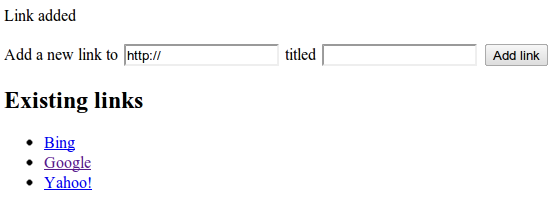
\includegraphics{13-yesods-monads-image-01.png}
\end{figure}

Пример: Запрос информации

Таким же образом вы можете получить информацию по звпросу внутри Widget. Здесь мы можем определить порядок сортировки списка на основе GET параметров.

\begin{lstlisting}
{-# LANGUAGE OverloadedStrings, TypeFamilies, TemplateHaskell,
             QuasiQuotes, TypeFamilies, MultiParamTypeClasses, GADTs #-}
import Yesod
import Data.Text (Text)
import Data.List (sortBy)
import Data.Ord (comparing)

data Person = Person
    { personName :: Text
    , personAge :: Int
    }

people :: [Person]
people =
    [ Person "Miriam" 25
    , Person "Eliezer" 3
    , Person "Michael" 26
    , Person "Gavriella" 1
    ]

data People = People

mkYesod "People" [parseRoutes|
/ RootR GET
|]

instance Yesod People

instance RenderMessage People FormMessage where
    renderMessage _ _ = defaultFormMessage


getRootR :: Handler RepHtml
getRootR = defaultLayout [whamlet|
<p>
    <a href="?sort=name">Sort by name
    \ | #
    <a href="?sort=age">Sort by age
    \ | #
    <a href="?">No sort
^{showPeople}
|]

showPeople :: Widget
showPeople = do
    msort <- lift $ runInputGet $ iopt textField "sort"
    let people' =
            case msort of
                Just "name" -> sortBy (comparing personName) people
                Just "age"  -> sortBy (comparing personAge)  people
                _           -> people
    [whamlet|
<dl>
    $forall person <- people'
        <dt>#{personName person}
        <dd>#{show $ personAge person}
|]

main :: IO ()
main = warpDebug 3000 People
\end{lstlisting}

Повторим, всё, что нужно сделать, это поднять (lift) наш нормальный код Handler (в данном случае, runInputGet), чтобы исполнить его в нашем Widget.

Выводы

Если вы полностью проигнорировали эту главу, вы все равно сможете использовать Yesod с большой пользой. Преимущество понимания того, как взаимодействуют монады Yesod, в том, чтобы иметь возможность производить более чистый, и более модульный код. Способность выполнять произвольные действия в Widget может быть мощным инструментом, и понимание того, как взаимодействуют Persistent и ваш код Handler может помочь вам сделать более обоснованные проектные решения в вашем приложении.
